\problemname{Miniröj}
De flesta som suttit vid en dator utan internet-uppkoppling har antagligen testat på att spela Minröj. Minröj spelas på en rektangulär spelplan med \texttt{RxC} stycken celler vars innehåll från början är okänt. Spelaren kan sedan klicka på cellerna för att se dess innehåll. I ett antal celler har minor placerats ut och klickar spelaren på en sådan så är spelet över. I varje cell utan mina finns istället en siffra som talar om hur många minor det finns i cellerna runtom, dvs i de celler med vilka den delar en sida eller ett hörn. Tanken är att dessa siffror ska användas för att lista ut var minorna finns och på så sätt undvika dem.

Rudolf har bestämt sig för att bli en professionell Minröj-spelare. Han har dock inte spelat det förut och tänker därför testa en lättare version, Miniröj, som spelas på ett spelbräde av storlek \texttt{2xN}. Han har dessutom laddat ner \emph{MinesweeperHaXX3000}, som genom att utnyttja en mystisk bugg kan avslöja innehållet i alla celler på den nedre halvan av spelplanen. Rudolf känner sig dock inte helt säker ändå, och ber dig att skriva ett program som givet den informationen han fått kan avgöra vilka celler som är säkra att klicka på.

\section*{Indata}
På den första och enda raden finns en sträng av längd $N$. Denna beskriver spelplanens nedre halva, och varje tecken är antingen ett '\texttt{X}', vilket innebär en mina, eller ett heltal $d$, $0 \leq d \leq 5$, som beskriver att det finns $d$ minor i närheten av rutan.

\section*{Utdata}
Om det inte finns någon giltig spelplan som är kompatibel med indata ska programmet skriva ut '\texttt{Fel i haxx}' på en rad (notera stor bokstav i början av raden). Skriv annars ut en sträng med $N$ tecken - '\texttt{S}', '\texttt{O}' eller '\texttt{X}' - beskrivande cellerna på den övre halvan av spelplanen. En cell beskrivs med '\texttt{S}' om cellen inte kan innehålla en mina, '\texttt{X}' om cellen helt säkert innehåller en mina och '\texttt{O}' om cellens innehåll inte går att avgöra.

\section*{Delpoäng}
\begin{itemize}
\item För 40\% av poängen gäller att $1 \leq N \leq 10 000$, och \emph{att det inte finns några minor i den nedre raden}.
\item För full poäng gäller att $1 \leq N \leq 50 000$.
\end{itemize}

\section*{Exempel}

\begin{figure}[h!]
\begin{center}
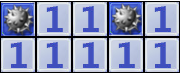
\includegraphics[scale=1]{miniroj1}
\end{center}
\caption{En illustration av en möjlig lösning för det första exempeltestfallet.}
\label{fig1}
\end{figure}

\begin{figure}[h!]
\begin{center}
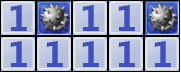
\includegraphics[scale=1]{miniroj2}
\end{center}
\caption{En illustration av den andra möjliga lösningen för det första exempeltestfallet.}
\label{fig1}
\end{figure}
